\message{ !name(latex_course.tex)}% Leslie Lamport hat LaTeX entwickelt, um dem Anwender das Schreiben
% spezieller Dokumente zu vereinfachen. Um den europäischen/deutschen
% Vorstellungen eines Layouts zu entsprechen, hat Markus Kohm analoge
% Dokumentklassen entwickelt (Koma-Klassen)

% Diese Dokumente sind
% im Original    extern              Koma       extern
% 1. article                         scrartcl
% 2. report                          scrreprt
% 3. book                            scrbook
% 4. letter                          scrlttr2
% 5. slide                                      beamer
% 6.             poster                         tikzposter
% 7.                                            komacv bzw. europecv
% Das Layout ist im Original amerikanischen Vorstellungen ensprechend!

% Der Aufbau ist immer

% Kopf des Dokumentes
% ===================
\documentclass[ngerman,               % in eckigen Klammern stehen
                                      % optionale Angaben, hier: ngerman
                                      % - es werden Trennmuster nach
                                      %   _n_euer deutscher Recht-
                                      %   schreibung geladen
                                      % - wenn das Zusatzpaket babel
                                      %   geladen ist, kann der Autor
                                      %   länderspezifische
                                      %   Befehle, beispielsweise für
                                      %   Anführungszeiche direkt
                                      %   eingeben
                                      % typographische Regeln:
                                      % in der scrreprt-Klasse beginnt
                                      % jedes Kapitel auf einer
                                      % neuen Seite, leere Seiten wie
                                      % die Zusammenfassung
                                      % erhalten keine Seitennummer,
                                      % ebensowenig Titelseiten, es
                                      % werden alle(!!!) Seiten intern
                                      % nummeriert, die Titelseite
                                      % hat die Nummer 1, die
                                      % Seitennummerierung erfolgt
                                      % unten mittig
               a4paper,               % Ausgabe auf DIN A4 Seiten
             % draft,                 % Satzspiegelfehler werden
                                      % angezeigt, Abbildungen werden
                                      % nicht ausgegeben
               fleqn,                 % math. Formeln werden mit festem
                                      % Einzug von links dargestellt
                     ]{scrreprt}

% Einstellungen
% =============

% Da die Einstellungen sich von Dokument zu Dokument kaum verändern,
% ist es sinnvoll, diese an einer zentralen Stelle abzulegen und von
% dort zu laden. Dies geschieht völlig transparent mit dem Befehl
% \input{<Pfad>}, dem als Argument eine Datei mit (relativem) Zugriffs-
% pfad übergeben wird
\input{../../shared/twp-cfg}
% in dieser Datei werden alle Zusatzpakete mittels
% \usepackage{<package>} geladen


% merke: ein späterer Titel überschreibt einen früher gesetzten Titel,
% in der scrreprt-Dokumentenklasse erscheint der Titel auf einer
% eigenen Seite
\title{Ein erstes \LaTeX-Dokument mit der Dokumentklasse \texttt{scrreprt}}
                         % \texttt{<Inhalt>} formatiert <Inhalt>
                         % mit einer dicktengleichen Schriftart
                         % im Vergleich zur ansonsten eingesetzten
                         % Proportionalschrift

% Rumpf des Dokumentes
\begin{document}

\message{ !name(latex_course.tex) !offset(864) }
Dieselbe Funktion \(f: \mathcal R \rightarrow \mathcal R\) mit \TeX{}
    als Datenprozessor:
\begin{verbatimwrite}{../../shared/figures/r_to_r_tex.tex}
  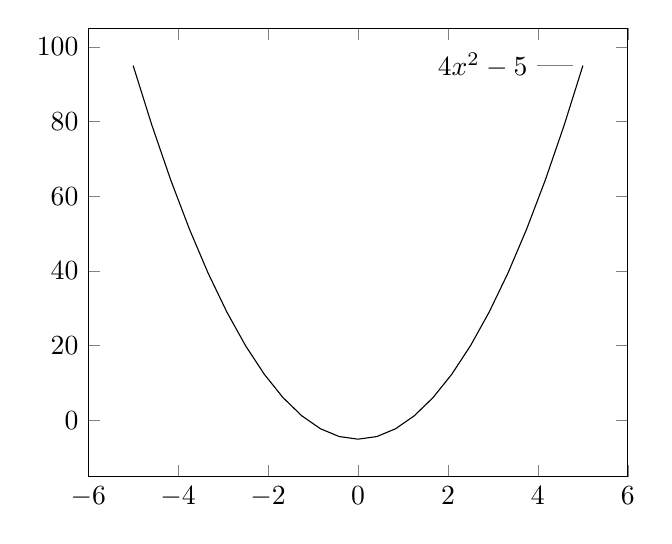
\begin{tikzpicture}
    \begin{axis}            % das Koordinatensystem wird mit der
                            % Umgebung axis erzeugt
      \addplot [            % ein Plot wird hinzugefügt
        domain=-5:5         % der Definitionsbereich
      ] { 4*x^2-5 }  % die Funktion
      node [pin=180:{$4x^2-5$}]{}; % Legende der Grafik
  \end{axis}
  \end{tikzpicture}
\end{verbatimwrite}
\lstinputlisting{../../shared/figures/r_to_r_tex.tex}

  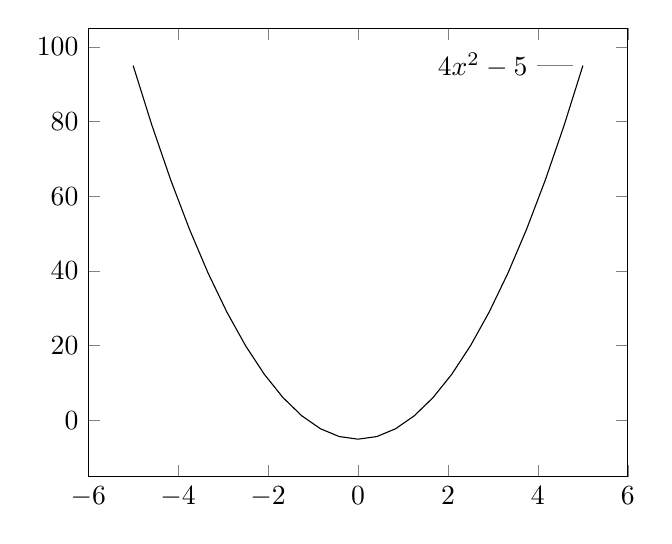
\begin{tikzpicture}
      \begin{axis}            % das Koordinatensystem wird mit
                              % der Umgebung axis erzeugt
          \addplot[             % ein Plot wird hinzugefügt
            domain=-5:5         % der Definitionsbereich
          ] { 4*x^2-5 }         % die Funktion
          node [pin=180:{$4x^2-5$}]{}; % Legende der Grafik
      \end{axis}
  \end{tikzpicture}

\message{ !name(latex_course.tex) !offset(963) }

\end{document}

% der folgende Kommentar wird vom Emacs gebraucht, ist also ansonsten ohne
% Bedeutung!

%%% Local Variables:
%%% mode: latex
%%% TeX-master: t
%%% TeX-engine: luatex
%%% ispell-local-dictionary: "deutsch8"
%%% End:
